\chapter{Preconditioners}

In this chapter, all preconditioners are presented. All preconditioners support local operators. They can be used as a global preconditioner via block-jacobi scheme which works locally on each interior matrix.

To provide fast application, all preconditioners require extra memory to keep the approximated operator.

\section{Code Structure}

The preconditioners provide a solution to the system $Mz=r$, where either the solution $z$ is directly computed by the approximation scheme or it is iterativily obtained with $z=0$ initial guess.

\begin{figure}[!ht]
\centering
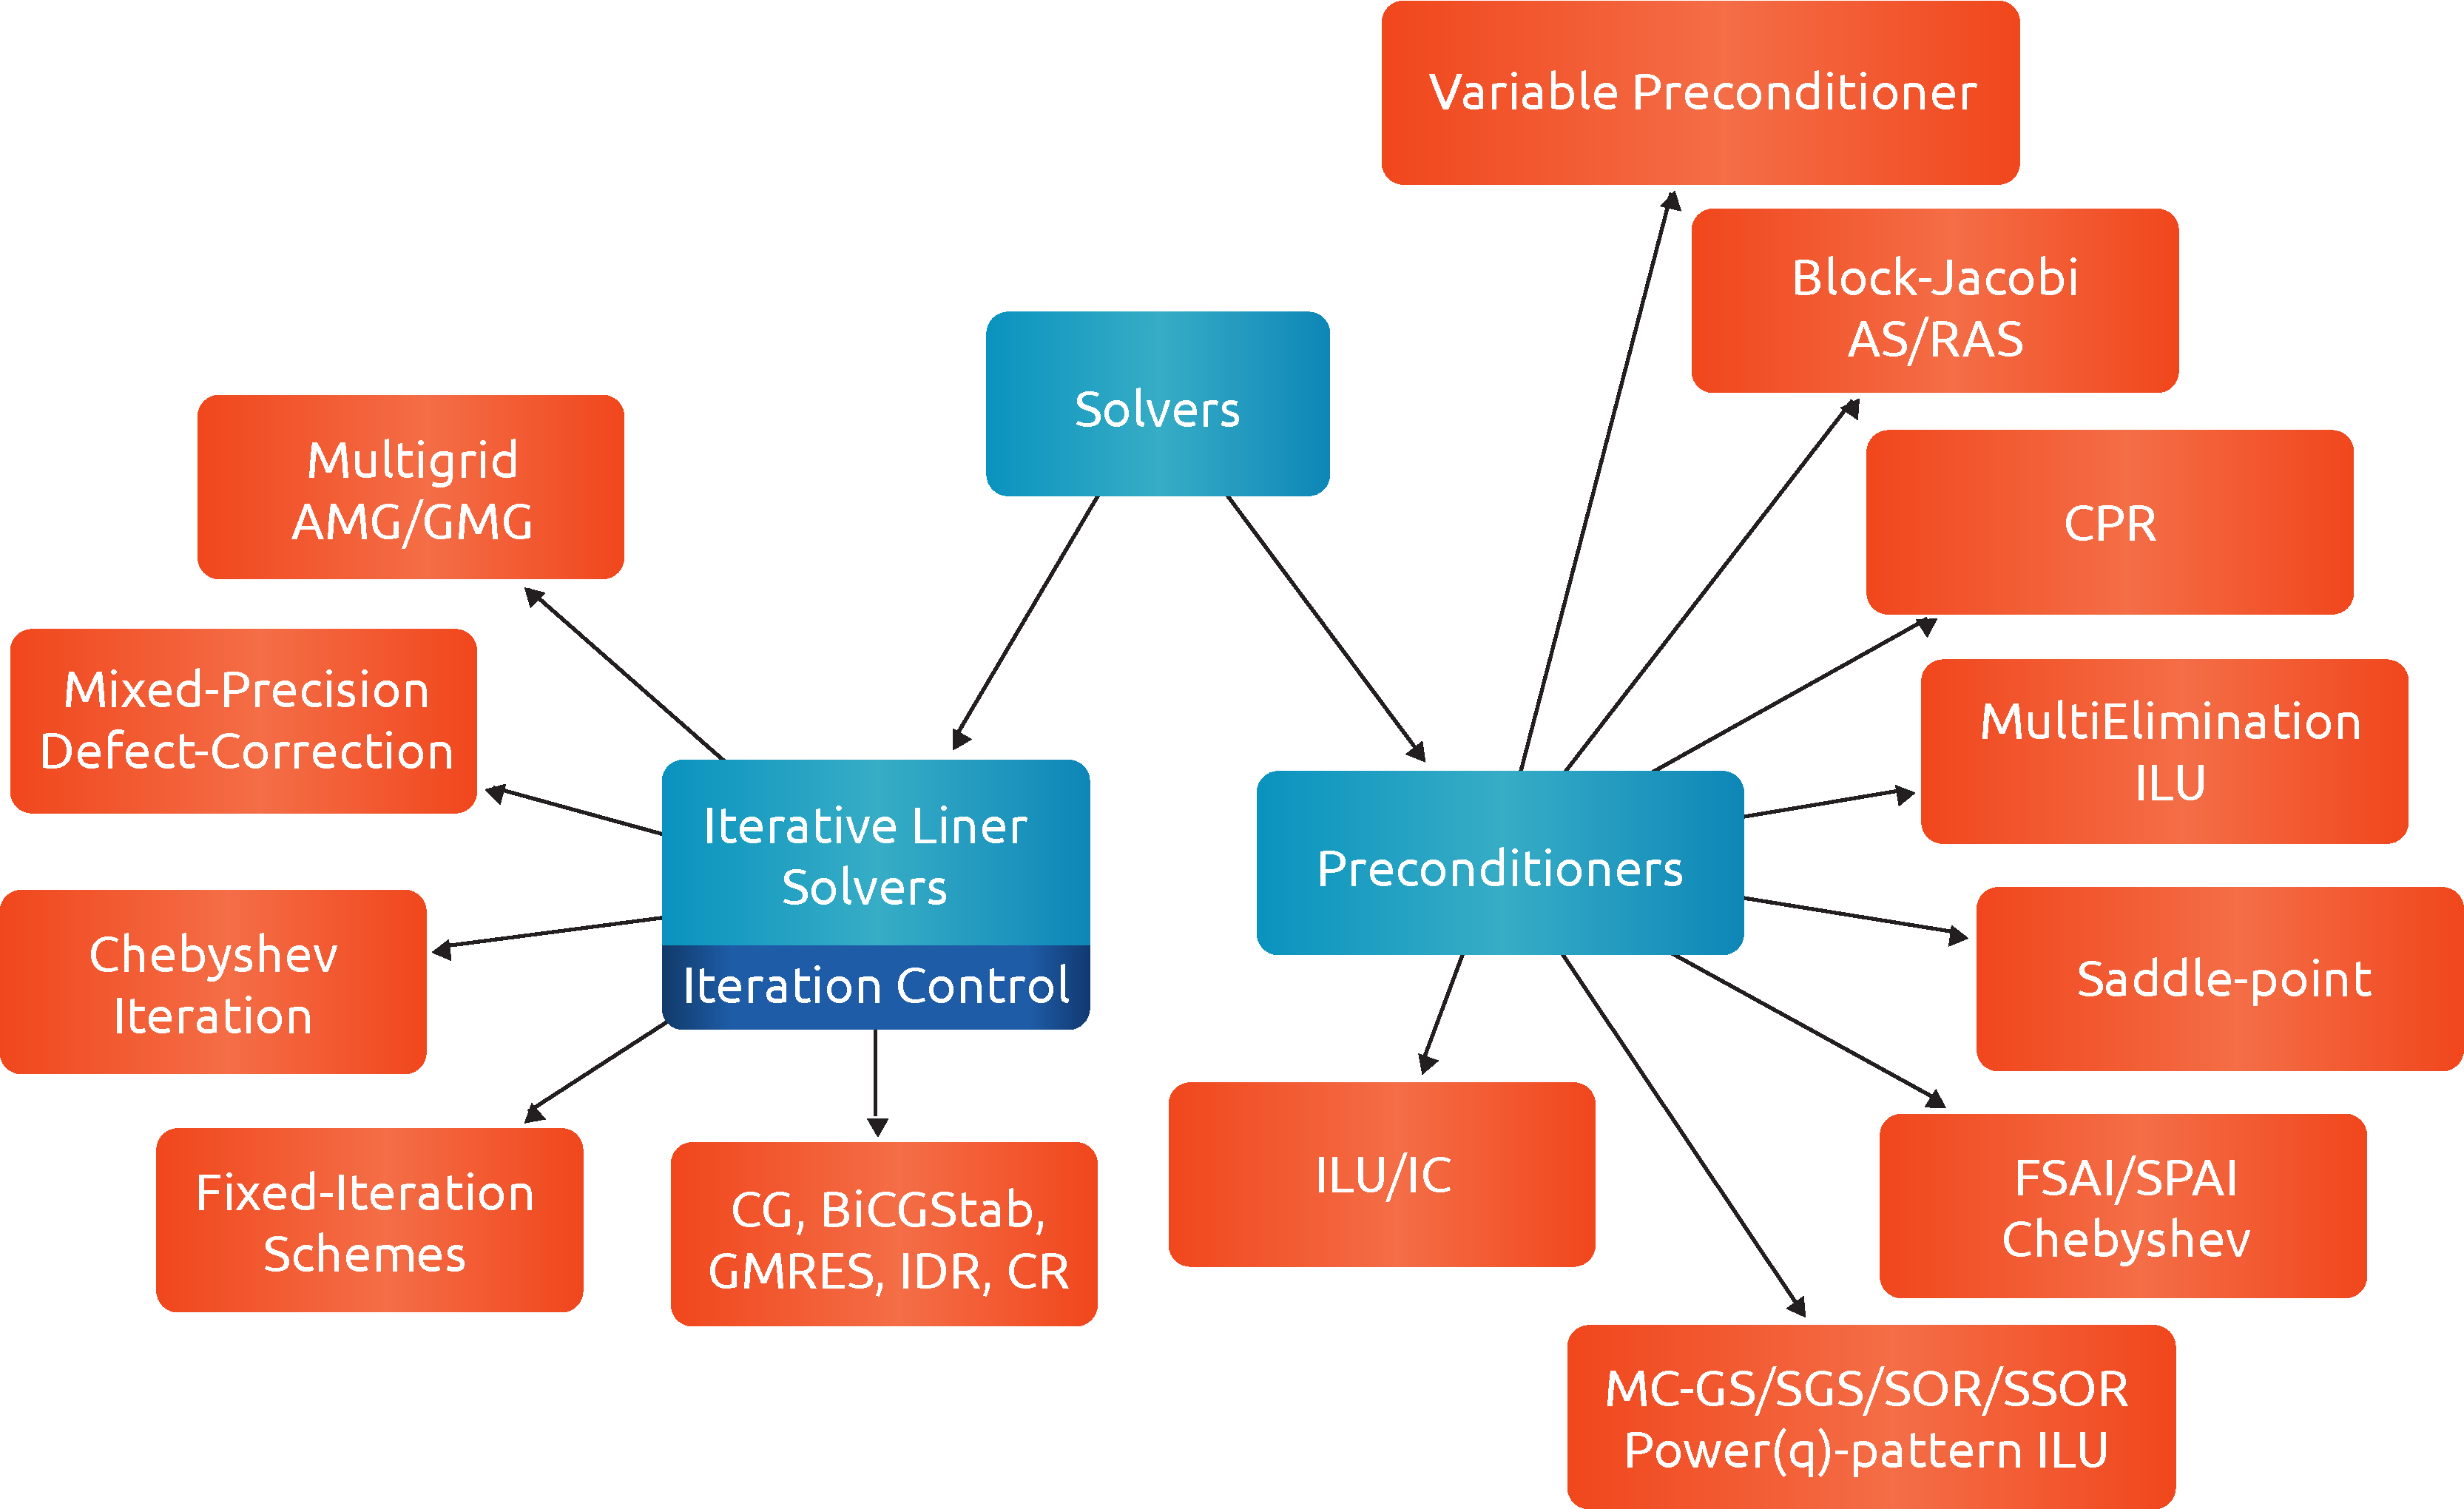
\includegraphics[width=0.95\textwidth]{./fig/solver.pdf}
\caption{Solver's classes hierarchy}
\label{paralution-solvers}
\end{figure}

\begin{figure}[!ht]
\centering
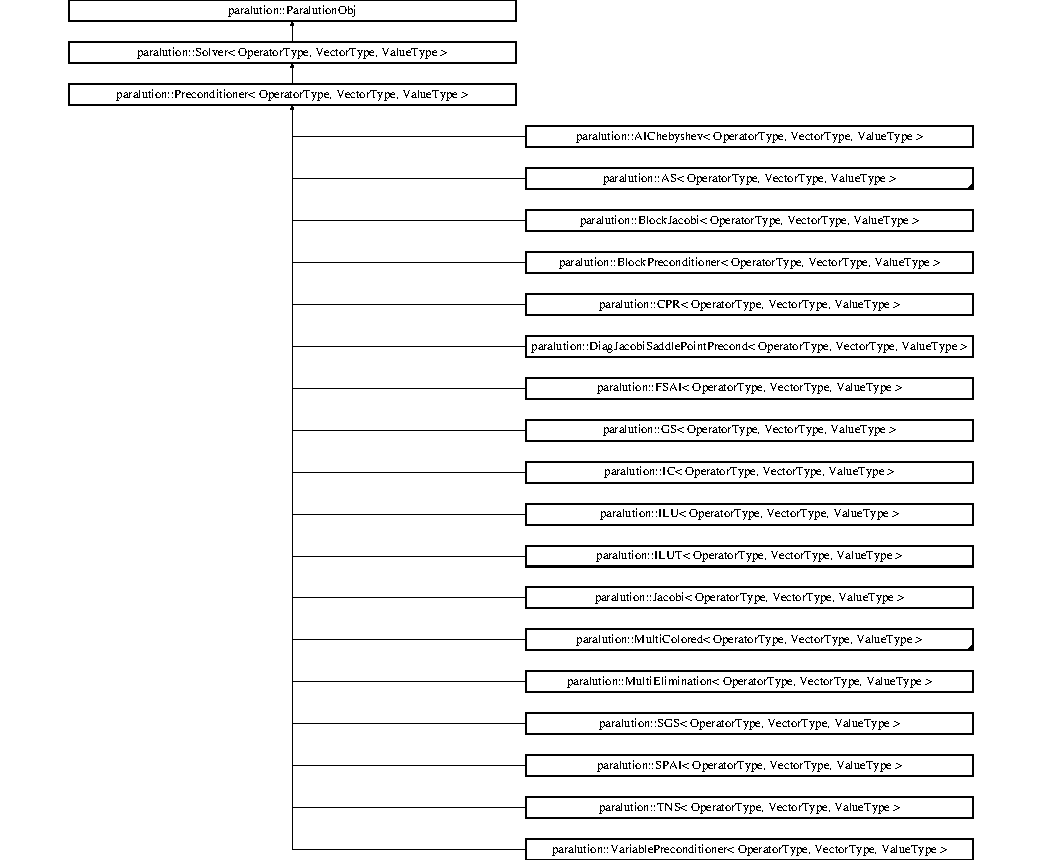
\includegraphics[width=0.99\textwidth]{./fig/body/classparalution_1_1_preconditioner.pdf}
\caption{Preconditioners}
\end{figure}

\section{Jacobi}

The Jacobi preconditioner is the simplest parallel preconditioner, details can be found in \cite{SAAD, templates, Demmel}.

\begin{table}[H]
\begin{tabular}{l|l|l|l}
\multicolumn{1}{c|}{ValueType} & Building phase & Solving phase & Available \\ \hline
D,F,C                          & H,C            & H,C,O,X       & S,M      
\end{tabular}
\end{table}


\lstinputlisting[title="Jacobi preconditioner"]{./src/pjac.cpp}


\section{Multi-colored (Symmetric) Gauss-Seidel and SOR}

\begin{table}[H]
\begin{tabular}{l|l|l|l}
\multicolumn{1}{c|}{ValueType} & Building phase & Solving phase & Available \\ \hline
D,F,C                          & H,C,           & H,C,O,X       & S,M      
\end{tabular}
\end{table}


The additive preconditioners are based on the splitting of the original matrix. Higher parallelism in solving the forward and backward substitution is obtained by performing a multi-colored decomposition. Details can be found in \cite{Lukarski2012, SAAD}.

\lstinputlisting[title="Multi-colored symmetric Gauss-Seidel preconditioner"]{./src/pgs.cpp}

\lstinputlisting[title="Multi-colored SOR with relaxation parameter 1.6"]{./src/pssor.cpp}


\section{Incomplete LU with levels -- ILU($p$)}

ILU($p$) factorization based on $p$-levels. Details can be found in \cite{SAAD}.

\begin{table}[H]
\begin{tabular}{l|l|l|l}
\multicolumn{1}{c|}{ValueType} & Building phase & Solving phase & Available \\ \hline
D,F,C                          & H              & H,C           & S,M      
\end{tabular}
\end{table}


\lstinputlisting[title="ILU(1) preconditioner - based on levels"]{./src/pilu.cpp}


\section{Incomplete Cholesky -- IC}


IC factorization without additional fill-ins. Details are given in \cite{SAAD}.

\begin{table}[H]
\begin{tabular}{l|l|l|l}
\multicolumn{1}{c|}{ValueType} & Building phase & Solving phase & Available \\ \hline
D,F,C                          & H              & H,C           & S,M      
\end{tabular}
\end{table}

\lstinputlisting[title="IC preconditioner"]{./src/pic.cpp}

\textbf{\emph{Note}} This implementation is still experimental and it is highly recommended to use the ILU
preconditioner instead.

\section{Incomplete LU with threshold -- ILUT($t$,$m$)}


Incomplete LU (ILUT($t$,$m$)) factorization based on threshold ($t$) and maximum number of elements per row ($m$). Details can be found in \cite{SAAD}. The preconditioner can be initialized with the threshold value only or with threshold and maximum number of elements per row. 

\begin{table}[H]
\begin{tabular}{l|l|l|l}
\multicolumn{1}{c|}{ValueType} & Building phase & Solving phase & Available \\ \hline
D,F,C                          & H              & H,C           & S,M      
\end{tabular}
\end{table}


\lstinputlisting[title="ILUT(0.01) preconditioner"]{./src/pilut.cpp}

\textbf{\emph{Note}} This implementation is still experimental.

\section{Power($q$)-pattern method -- ILU($p$,$q$)}

ILU($p$,$q$) is based on the ILU($p$) factorization with a power($q$)-pattern method, the algorithm can be found in\cite{Lukarski2012}. This method provides a higher degree of parallelism of forward and backward substitution compared to the standard ILU($p$) preconditioner.

\begin{table}[H]
\begin{tabular}{l|l|l|l}
\multicolumn{1}{c|}{ValueType} & Building phase & Solving phase & Available \\ \hline
D,F,C                          & H,C            & H,C,O,X       & S,M      
\end{tabular}
\end{table}

\textbf{\emph{Note}} If the preconditioner is initialized with only the first argument ($p$) then $q$ is taken to be $p+1$. 

\lstinputlisting[title="ILU(1 2) preconditioner - based on power($q$)-pattern method"]{./src/pmcilu.cpp}

\section{Multi-Elimination ILU}

The multi-elimination ILU preconditioner is based on the following decomposition
\begin{eqnarray}
A =\left[
\begin{array}{cc}  
D & F \\ 
E & C 
\end{array}\right]
= \left[
\begin{array}{cc}  
I & 0 \\ 
E D^{-1} & I 
\end{array}\right]
\times \left[
\begin{array}{cc}  
D & F \\ 
0 & \hat{A}
\end{array}\right],
\end{eqnarray}
where $\hat{A}=C - E D^{-1} F$.\\

To make the inversion of $D$ easier, we permute the preconditioning before the factorization with a permutation $P$ to obtain only diagonal elements in $D$. The permutation here is based on a maximal independent set. Details can be found in \cite{SAAD}.


This procedure can be applied to the block matrix $\hat{A}$, in this way we can perform the factorization recursively. In the last level of the recursion, we need to provide a solution procedure. By the design of the library, this can be any kind of solver. In the following example we build a preconditioned CG solver with a multi-elimination preconditioner defined with 2 levels and without drop-off tolerance. The last block of preconditioner is solved using a Jacobi preconditioner.

\begin{table}[H]
\begin{tabular}{l|l|l|l}
\multicolumn{1}{c|}{ValueType} & Building phase & Solving phase & Available \\ \hline
D,F,C                          & H,C            & H,C,O         & S,M      
\end{tabular}
\end{table}

\lstinputlisting[title="PCG solver with multi-elimination ILU preconditioner and Jacobi"]{./src/me-ilu.cpp}

\section{Diagonal Preconditioner for Saddle-Point Problems}

Consider the following saddle-point problem
\begin{eqnarray}
A =\left[
\begin{array}{cc}  
K & F \\ 
E & 0 
\end{array}\right].
\end{eqnarray}

For such problems we can construct a diagonal Jacobi-like preconditioner of type
\begin{eqnarray}
P =\left[
\begin{array}{cc}  
K & 0 \\ 
0 & S 
\end{array}\right]
\end{eqnarray}
with $S=E D^{-1} F$, where $D$ are the diagonal elements of $K$.\\

The matrix $S$ is fully constructed (via sparse matrix-matrix multiplication). 

The preconditioner needs to be initialized with two external solvers/preconditioners -- one for the matrix $K$ and one for the matrix $S$. 

\begin{table}[H]
\begin{tabular}{l|l|l|l}
\multicolumn{1}{c|}{ValueType} & Building phase & Solving phase & Available \\ \hline
D,F,C                          & H,C            & H,C,O,X       & S,M      
\end{tabular}
\end{table}

\lstinputlisting[title="GMRES solver with diagonal Jacobi-like preconditioner for Saddle-Point problems"]{./src/djsdp.cpp}


\section{Chebyshev Polynomial}

The Chebyshev approximate inverse matrix is based on the work \cite{chebpoly}.

\begin{table}[H]
\begin{tabular}{l|l|l|l}
\multicolumn{1}{c|}{ValueType} & Building phase & Solving phase & Available \\ \hline
D,F,C                          & H,C            & H,C,O,X       & S,M      
\end{tabular}
\end{table}

\lstinputlisting[title="Chebyshev polynomial preconditioner"]{./src/cheb.cpp}


\section{FSAI($q$)}

The Factorized Sparse Approximate Inverse preconditioner computes a direct approximation
of $M^{-1}$ by minimizing the Frobenius norm $||I-GL||_F$ where $L$ denotes the
exact lower triangular part of $A$ and $G:=M^{-1}$. The FSAI preconditioner is
initialized by $q$, based on the sparsity pattern of $\left|A\right|^q$ \cite{Lukarski2012}. 
However, it is also possible to supply external sparsity patterns in form of the LocalMatrix class.
Further details on the algorithm are given in~\cite{kolotilina}.

\begin{table}[H]
\begin{tabular}{l|l|l|l}
\multicolumn{1}{c|}{ValueType} & Building phase & Solving phase & Available \\ \hline
D,F,C                          & H              & H,C,O,X       & S,M      
\end{tabular}
\end{table}

\lstinputlisting[title="FSAI(2) preconditioner"]{./src/pfsai.cpp}

\textbf{\emph{Note}} The FSAI(q) preconditioner is only suited for SPD matrices.

\section{SPAI}

The SParse Approximate Inverse algorithm is an explicitly computed preconditioner for
general sparse linear systems. In its current implementation, only the sparsity pattern
of the system matrix is supported. The SPAI computation is based on the minimization of
the Frobenius norm $||AM - I||_F$. Details can be found in~\cite{grote}.

\begin{table}[H]
\begin{tabular}{l|l|l|l}
\multicolumn{1}{c|}{ValueType} & Building phase & Solving phase & Available \\ \hline
D,F,C                          & H              & H,C,O,X       & S,M      
\end{tabular}
\end{table}

\lstinputlisting[title="SPAI preconditioner"]{./src/pspai.cpp}

\textbf{\emph{Note}} The SPAI implementation is still experimental. The current version is based on a original static matrix pattern (similar to ILU0).

\section{Block Preconditioner}

When handling vector fields, typically one can try to use different preconditioners/solvers for the different blocks. For such problems, the library provides a block-type preconditioner. This preconditioner builds the following block-type matrix

\begin{eqnarray}
P =\left[
\begin{array}{cccc}  
A_d & 0   & . & 0\\ 
B_1 & B_d & . & 0\\
.   & .   & . & .\\
Z_1 & Z_2 & . & Z_d\\
\end{array}\right]
\end{eqnarray}

The solution of $P$ can be performed in two ways. It can be solved by block-lower-triangular sweeps with inversion of the blocks $A_d$...$Z_d$ and with a multiplication of the corresponding blocks, this is set by the function \emph{SetLSolver()} (which is the default solution scheme). Alternatively, it can be used only with an inverse of the diagonal $A_d$...$Z_d$ (such as Block-Jacobi type) by using the function \emph{SetDiagonalSolver()}. 

\begin{table}[H]
\begin{tabular}{l|l|l|l}
\multicolumn{1}{c|}{ValueType} & Building phase & Solving phase & Available \\ \hline
D,F,C                          & H,C            & H,C,O,X       & S,M      
\end{tabular}
\end{table}

\lstinputlisting[title="Block Preconditioner for two MC-ILU"]{./src/block-precond.cpp}
\lstinputlisting[title="Block Preconditioner for MC-ILU and AMG"]{./src/block-precond2.cpp}

\section{Additive Schwarz and Restricted Additive Schwarz -- AS and RAS}

As a preconditioning technique, we can decompose the linear system $Ax=b$ into small sub-problems based on
%
\begin{eqnarray}
A_i=R_i^T A R_i
\end{eqnarray}
% 
where $R_i$ are restriction operators. Thus, we can define:

\begin{itemize}
\itemsep0em

\item{Additive Schwarz (AS)} -- the restriction operators produce sub-matrices which overlap. This leads to contributions from two preconditioners on the overlapped area, see Figure~\ref{blockprecond} (left). Thus these contribution sections are scaled by $1/2$.

\item{Restricted Additive Schwarz (RAS)} -- this is a mixture of the pure block-Jacobi and the additive Schwarz scheme. Again, the matrix $A$ is decomposed into squared sub-matrices. The sub-matrices are large as in the additive Schwartz approach -- they include overlapped areas from other blocks. After we solve the preconditioning sub-matrix problems, we provide solutions only to the non-overlapped area, see Figure~\ref{blockprecond} (right).
\end{itemize}

\begin{table}[H]
\begin{tabular}{l|l|l|l}
\multicolumn{1}{c|}{ValueType} & Building phase & Solving phase & Available \\ \hline
D,F,C                          & H,C            & H,C,O,X       & S,M      
\end{tabular}
\end{table}


\begin{figure}[h]
\centering
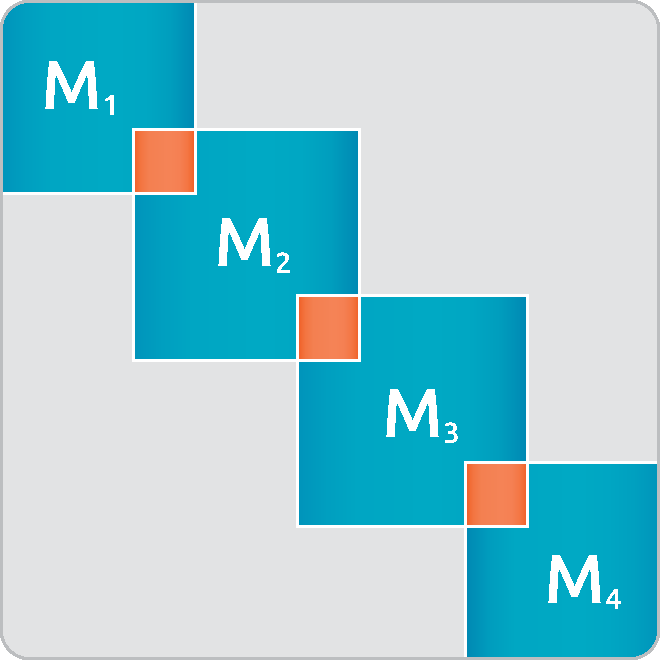
\includegraphics[width=0.31\textwidth]{./fig/AS}
\hspace{10mm}
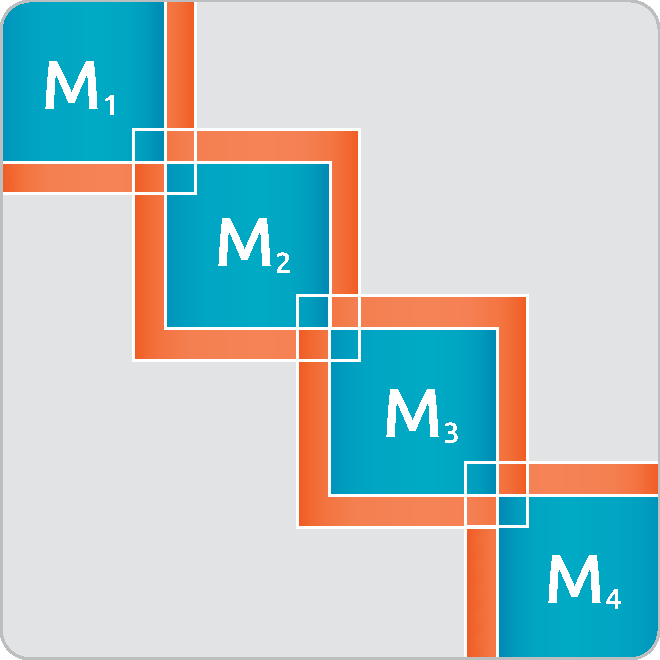
\includegraphics[width=0.31\textwidth]{./fig/RAS}
\caption{Example of a 4 block-decomposed matrix -- Additive Schwarz (AS) with overlapping preconditioner (left) and Restricted Additive Schwarz (RAS) preconditioner (right)}
\label{blockprecond}
\end{figure}

Details can be found in \cite{SAAD,RAS,Quarteroni1999,Smith1996,Toselli2005}.

The library provides Additive Schwarz (called \emph{AS}) and Restricted Additive Schwarz (called \emph{RAS}) preconditioners. For both preconditioners, the user need to to specify the number of blocks, the size of the overlapping region and the type of preconditioners which should be used on the blocks.

\lstinputlisting[title="(Restricted) Additive Schwarz defined with 3 blocks and 10 overlapping elements"]{./src/as-precond.cpp}

\section{Truncated Neumann Series Preconditioner (TNS)}

The Truncated Neumann Series Preconditioner (TNS) is based on
\begin{eqnarray}
M^{-1} = K^T D^{-1} K,
\end{eqnarray}

where $K = (I - LD^{-1} + (LD^{-1})^2)$, $D$ is the diagonal matrix of $A$ and $L$ is strictly the lower triangular part of $A$.

The preconditioner can be computed in two forms - explicitly and implicitly. In the implicit form, the full construction of $M$ is performed via matrix-matrix operations. Whereas in the explicit from, the application of the preconditioner is based on matrix-vector operations only. The matrix format for the stored matrices can be specified.

\begin{table}[H]
\begin{tabular}{l|l|l|l}
\multicolumn{1}{c|}{ValueType} & Building phase & Solving phase & Available \\ \hline
D,F,C                          & H,C            & H,C,O,X       & S,M      
\end{tabular}
\end{table}

\lstinputlisting[title="Truncated Neumann Series Preconditioner (TNS)"]{./src/tns.cpp}


\section{Variable Preconditioner}

The Variable Preconditioner can hold a selection of preconditioners. In this way any type of preconditioners can be combined. As example, the variable preconditioner can combine Jacobi, GS and ILU -- then, the first iteration of the iterative solver will apply Jacobi, the second iteration will apply GS and the third iteration will apply ILU. After that, the solver will start again with Jacobi, GS, ILU. It is important to be used with solvers which can handle such type of preconditioners.

\begin{table}[H]
\begin{tabular}{l|l|l|l}
\multicolumn{1}{c|}{ValueType} & Building phase & Solving phase & Available \\ \hline
D,F                            & H,C,O          & H,C,O         & S,M      
\end{tabular}
\end{table}


\section{CPR Preconditioner}

\begin{flushright}
{\color{red} This preconditioner is still under development and it is not part of the official distributions}
\end{flushright}

The CPR (Constrained Pressure Residual) preconditioner is a special type of preconditioner for reservoir simulations. The preconditioner contains two (or three) stage sub-preconditioners. 

\begin{table}[H]
\begin{tabular}{l|l|l|l}
\multicolumn{1}{c|}{ValueType} & Building phase & Solving phase & Available \\ \hline
D,F,C                          & H,C,O,X        & H,C,O,X       & S,M      
\end{tabular}
\end{table}

The user has the ability to select any combination of the two (or three) sub-preconditioners, as well as to use the default ILU-like and AMG configuration.


\section{MPI Preconditioners}

The MPI preconditioners are designed to work in parallel on all MPI processes. In this way, any type of preconditioner can be wrapped in a Block-Jacobi type, where the preconditioner will be applied locally on each interior matrix.

\begin{table}[H]
\begin{tabular}{l|l|l|l}
\multicolumn{1}{c|}{ValueType} & Building phase & Solving phase & Available \\ \hline
D,F,C                          & H,C,O          & H,C,O         & M      
\end{tabular}
\end{table}




